Depending on the application the Space Segment of a mission can vary in an infinite number of ways. Probably the most famous and widely used satellite constellation is the the Global Positioning System satellite network. In this case, it uses an irregular geometry.
\\
\\
\textbf{The GPS Constellation: An example of irregular distributed orbits \cite{GPS}}
\\
The GPS is a constellation property of the U.S. It provides positioning, navigation and timing. The constellation was designed with a 24-slot arrangement to ensure a visibility of at least four satellites from any point on the planet. Nowadays the constellation has expanded to a total operative number of 27-slot since June 2011. Some characteristic parameters of the satellites are the following:

\begin{itemize}
\item Orbit: Almost Circular
\item Height = 20,200 km (MEO);
\item Lifetime = 12.5 years;
\item Satellite Cost = 166 million USD;
\item Inclination = 55º;
\item Number of planes = 6;
\item Phasing: 30º-105º-120º-105º;
\end{itemize}

\begin{figure}[H]
\begin{center}
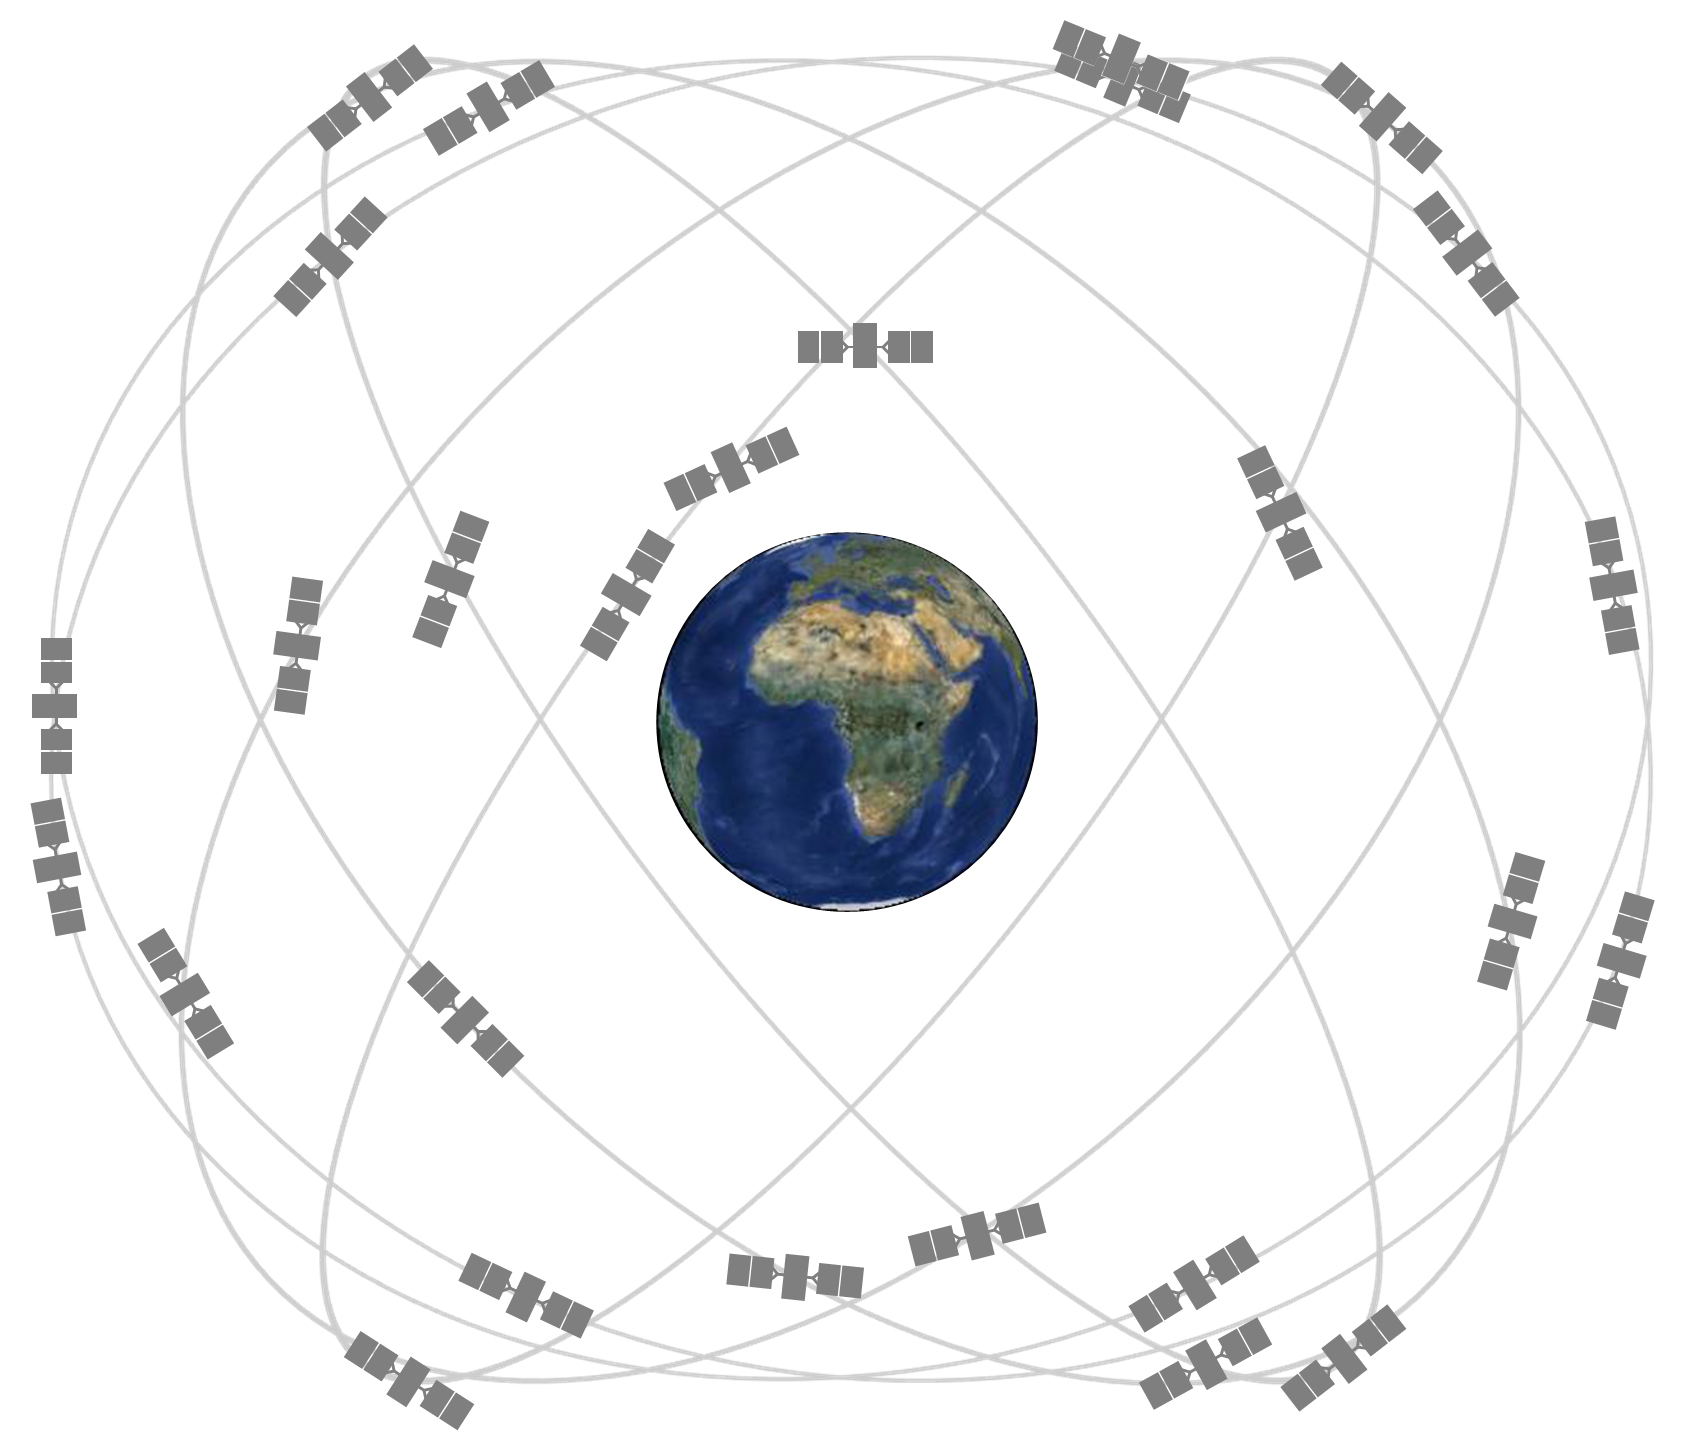
\includegraphics[scale=0.16]{GPSconstellation.jpg}
\caption{Distribution of the expanded 24-slot GPS constellation.\cite{GPS}}
\end{center}
\end{figure}